% Project Specifications

\chapter{Hardware Architecture}

\section{Hardware Resources}

The development board for this project is Nexys 4 from Digilent with an Artix-7 \gls{fpga} chip from Xilinx.
Table \ref{table:hardware_resources} summarizes the hardware resources available on the Nexys 4 board.

% [h] means here, can use [h!] to override internal LaTeX parameters
\begin{table}[h]
  \centering
  \caption{Nexys 4 Resource Specifications}
  \begin{tabular}{l | l}
    Logic Slices & 15850 \\
    Block RAM & 4860 Kbits \\
    DSP Slices & 240 \\
    Cellular RAM & 16MB \\
    Quad-SPI Flash & 16MB
  \end{tabular}
  \label{table:hardware_resources}
\end{table}

\section{Calculate Memory Requirement}

\gls{bram} will be the main active memory for input, output, weight, and bias data. The \gls{fpga} chip in use
contains 4860 Kbits of \gls{bram}, which is 607.5KB. The original model size is around 13.7MB, which is
considered very compact when compared with other deep learning models but still very demanding for
our system. Once quantized, the model size is roughly 3.5MB. So it is not possible to fit the entire model
into the \gls{bram} and it is inevitable to interact with external storage devices, e.g., the 16MB Quad-SPI
Flash or the 16MB \gls{psram} on the Nexys 4 board.

Because the resources on the board is quite limited, it is easiest to compute the model in a layer-by-layer
fasion without exploiting the layer-wise parallelism. First, the weights of a transposed
convolutional layer are read from the external storage device, the layer is then computed, followed by one or
more auxiliary layers such as batch normalization or activation layer. The output is then transfered from
the output \gls{bram} buffer to the input \gls{bram} buffer, then the weights of the next transposed
convolutional layer are read and the process continues until it reaches the final layer.

In order to allocate \gls{bram} properly, it is necessary to list the detailed memory requirements of each
layer.

\begin{table}[h]
  \centering
  \caption{Memory Requirement by Layers}
  \begin{tabular}{l | l | l | l | l}
    \toprule
    Layer & Input & Weight & Bias & Output \\
    \midrule
    1 & 100(8) & 819200(8) & 512(32) & 8192(32) \\
    2 & 8192(32) & 512(32) & 512(32) & 8192(32) \\
    3 & 8192(32) & - & - & 8192(8) \\
    4 & 8192(8) & 2097152(8) & 256(32) & 16384(32) \\
    5 & 16384(32) & 256(32) & 256(32) & 16384(32) \\
    6 & 16384(32) & - & - & 16384(8) \\
    7 & 16384(8) & 524288(8) & 128(32) & 32768(32) \\
    8 & 32768(32) & 128(32) & 128(32) & 32768(32) \\
    9 & 32768(32) & - & - & 32768(8) \\
    10 & 32768(8) & 131072(8) & 64(32) & 65536(32) \\
    11 & 65536(32) & 64(32) & 64(32) & 65536(32) \\
    12 & 65536(32) & - & - & 65536(8) \\
    13 & 65536(8) & 3072(8) & 3(32) & 12288(32) \\
    14 & 12288(32) & - & - & 12288(8) \\
    \bottomrule
  \end{tabular}
  \label{table:memory_requirements}
\end{table}

In table \ref{table:memory_requirements}, the numbers in parentheses are the bit width of the values. The table
indicates the maximum input/output size is 65536 in 32-bit, the maximum weight size is 2097152 in 8-bit, the
maximum bias size is 512 in 32-bit. However, notice that when both input is 65536 in 32-bit, the corresponding
layers are batch normalization and ReLU. This means that the same buffer can be used to store both the
input and output because the input can be updated in-place. Consequently the input buffer only needs to
store 65536 values in 8-bit.

To conclude, four main buffers are needed: input buffer (65536 bytes), output buffer (262144 bytes),
weight buffer (2097152 bytes), bias buffer (16384 bytes). Some auxiliary buffers are needed to store
the quantization parameters.

\section{Architecture}

The system stores weights of transposed convolutional layer in the 16MB Quad-SPI Flash. A computation unit
contains a transposed convolution module TC, a batch normalization module BN, a ReLU module ReLU,
and a tanh module Tanh. The unit can be configured to be TC-BN-ReLU or TC-Tanh. The network computes one
layer at a time. Before reading the final layer, the output of the computation unit is transferred to the
input buffer. The final result is sent to computer via \gls{uart} (serial port). Figure
\ref{fig:computation_unit} shows the structure of the computation unit.

\begin{figure}[h]
  \centering
  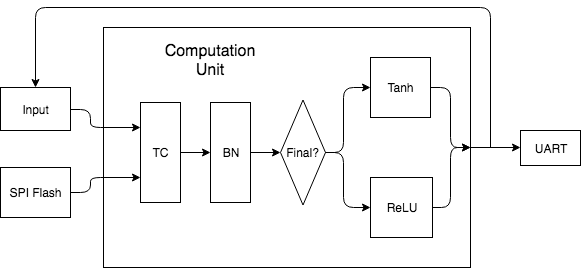
\includegraphics[scale=0.75]{computation_unit}
  \caption{Computation Unit Block Diagram}
  \label{fig:computation_unit}
\end{figure}

The input of the TC module are quantized 8-bit integers, while the output of the TC module are 32-bit
integers, which are input to the BN module. The BN first dequantizes the 32-bit input to 32-bit
single-precision floating-point numbers according to IEEE 754 standard, then the computation is carried
out in floating-point and the results are feed to the ReLU module, which simply sets negative values to
$0.0$ and then quantizes the output to 8-bit integers again and overwrites the input buffer with the
results. When the flow reaches the final Tanh module, the 32-bit input integers are dequantized just as the
BN module, $tanh$ is then performed on the floating-point numbers, and the final floating-point result is
sent to the computer through \gls{uart}, which can then be displayed with a simple conversion script.

\clearpage %force the next chapter to start on a new page. Keep that as the last line of your chapter!
